\subsection{ASL-Phono}
\label{sec:metodologia-datasets-phono}

% TODO revisar esta introdução
O ASL-Phono, por sua vez, introduz uma nova representação baseada na linguística, que descreve os sinais do \acrshort{asllvd} em termos de um conjunto de atributos da fonologia da \acrshort{asl}.

Ele é originado a partir das coordenadas 3D fornecidas para as 9.747 amostras do ASL-Skeleton3D e computando os respectivos atributos fonológicos, conforme descrito nas seções a seguir.

Entre os parâmetros fonológicos discutidos na \autoref{sec:linguistica-fonologia}, quatro foram selecionados para compor essa primeira versão do ASL-Phono, que são: configuração de mão, orientação, movimento e uma expressão não-manual referente à abertura da boca do sinalizador.

Dessa forma, analisemos adiante os passos utilizados para computá-los:

\begin{enumerate}
    \item \textbf{Configuração de mão}: refere-se à configurações das mãos do sinalizador durante a articulação dos sinais.
    O \acrshort{asllvd} fornece a configuração de mão inicial e final para cada um de seus sinais, a qual é definida dentre 88 opções apresentadas pelo \acrfull{asllrp}\footnote{Disponível em \url{http://www.bu.edu/asllrp}} \cite{neidle-2020-asllrp}.

    Utilizamos essa informação como base para computar as configurações de mãos no ASL-Phono, mas tivemos que adotar um passo extra para que pudéssemos atribuir configurações a todos os frames das amostras a partir dessas duas únicas providas. Nesse caso, dividimos os frames em duas metades: a primeira, contendo os frames iniciais do sinal, recebeu a configuração de mão inicial provida pelo \acrshort{asllvd}; a segunda, referente aos frames restantes finais, recebeu a configuração final provida.

    % -----
    \item \textbf{Orientação}: refere-se à direção para qual as palmas das mãos apontam durante a articulação dos sinais.
    Para calculá-la, utilizamos um pouco de álgebra linear e exploramos a relação das mãos para com o espaço tridimensional em que suas coordenadas estão representadas \cite{anton-2013-algebra}.

    Para isso, primeiro assumimos cada palma como sendo um plano que atravessa as coordenadas estimadas para as mãos (vide \autoref{subfig:palm-orientation}). A partir disso, selecionamos três coordenadas para descrever este plano: \(W\), que corresponde à coordenada do pulso; \(L\), localizada na base do dedo mínimo; e \(I\), localizada na base do dedo indicador.

    \begin{figure}[ht!]
        \centering
        \caption{
            \textmd{As coordenadas \(W\), \(L\) e \(I\) e os vetores auxiliares são utilizados para obter a normal \(\protect \overrightarrow{n}\) da palma da mão~(\subref{subfig:palm-orientation}).
            A direção da palma \(O_{palm}\) é então calculada a partir de \(\protect \overrightarrow{n}\) e descrita dentre um conjunto de direções possíveis~(\subref{ subfig:palm-directions}).}
        }
        \subcaptionbox{\label{subfig:palm-orientation}}{
            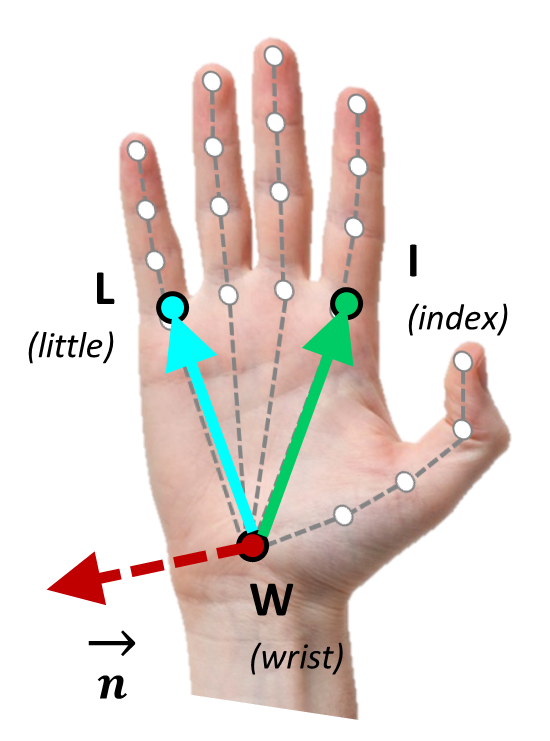
\includegraphics[height=4cm]{imagens/metodologia/datasets/palm_orientation_algebra}
        }%
        \hspace{1cm}
        \subcaptionbox{\label{ subfig:palm-directions}}{
            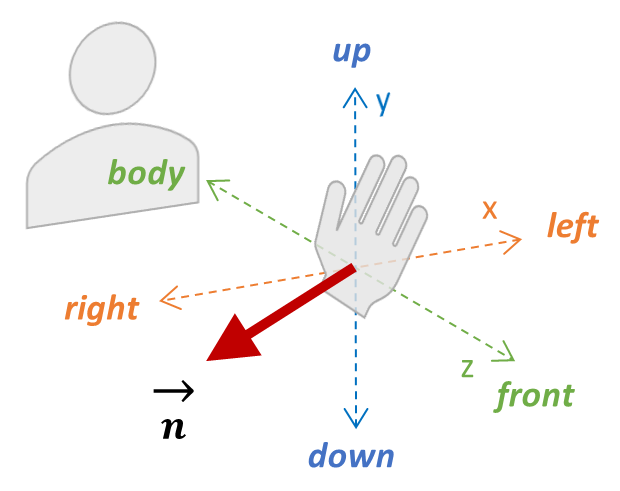
\includegraphics[height=4cm]{imagens/metodologia/datasets/hand_orientations}
        }%
        \nomefonte{}
        \label{fig:palm-orientation-directions}
    \end{figure}

    Por meio dessas coordenadas, é possível estabelecer dois vetores para descrever o plano da palma (vide \autoref{subfig:palm-orientation}): \(\overrightarrow{WL}\), indicado pela seta azul e \(\overrightarrow{WI}\), indicado pela seta verde. Através deles, é possível estabelecer o vetor normal \(\overrightarrow{n}\) perpendicular ao plano da palma, que é indicado pela seta vermelha tracejada, e calculado conforme \autoref{eqn:normal-palm-left} (para a mão esquerda) e \autoref{eqn:normal-palm-right} (para a mão direita):

    % Palm orientation:
    \begin{equation}
        \label{eqn:normal-palm-left}
        \overrightarrow{n}_{left} = \overrightarrow{WI} \times \overrightarrow{WL}
    \end{equation}

    \begin{equation}
        \label{eqn:normal-palm-right}
        \overrightarrow{n}_{right} = \overrightarrow{WL} \times \overrightarrow{WI}
    \end{equation}


    Finalmente, ao avaliar os valores dos eixos \(x\), \(y\) e \(z\) da normal \(\overrightarrow{n}\), é possível definir a orientação da palma \(O_{palm}\) como sendo a combinação de até três direções, cujas opções são: \textit{right} (direita), \textit{left} (esquerda), \textit{up} (para cima), \textit{down} (para baixo), \textit{body} (para o corpo) ou \textit{front} (para frente).
    Por exemplo, ``\textit{right\_down}'' e ``\textit{left\_up\_body}'' seriam orientações válidas. Essa avaliação é realizada conforme \autoref{eqn:palm-orientation-directions}:
    
    % Directions
    \begin{equation}
        \label{eqn:palm-orientation-directions}
        O_{palm} =
        \begin{cases}
            right & \text{if $\overrightarrow{n}_x < {-k}$ } \\
            left  & \text{if $\overrightarrow{n}_x > {k}$ }  \\
            up    & \text{if $\overrightarrow{n}_y < {-k}$ } \\
            down  & \text{if $\overrightarrow{n}_y > {k}$ }  \\
            body  & \text{if $\overrightarrow{n}_z < {-k}$ } \\
            front & \text{if $\overrightarrow{n}_z > {k}$ }  \\
        \end{cases}
    \end{equation}

    Onde o limiar \(k\) é definido empiricamente como 0,30 para filtrar variações pouco significativas em \(\overrightarrow{n}\). Observe na \autoref{ subfig:palm-directions} como essa operação é aplicada no espaço tridimensional à frente do sinalizador.


    % -----
    \item \textbf{Movimento}: descreve o deslocamento realizado pelas mãos na articulação do sinal.
    De forma semelhante ao que fizemos para a orientação da palma, aqui também analisaremos coordenadas das mãos para determinar sua trajetória no espaço.

    Para isso, utilizaremos a coordenada \(M\) como ponto de referência para as mãos, a qual está localizada na base do dedo médio (vide \autoref{fig:hand-movement-directions}). Com base nela, calcularemos o deslocamento ocorrido entre os frames anterior (tempo \(t-1\)) e atual (tempo \(t\)) para determinar o vetor de movimento \(\overrightarrow{m}\) (indicado pela seta vermelha tracejada), conforme \autoref{eqn:hand-movement}:
    
    % Movement of the hands:
    \begin{equation}
        \label{eqn:hand-movement}
        \overrightarrow{m} = M_{t} - M_{t-1}
    \end{equation}

    \begin{figure}[ht!]
        \centering
        \caption{
            \textmd{O vetor de movimento \(\protect \overrightarrow{m}\) é calculado pela trajetória da coordenada \(M\) entre os frames anterior (\(t-1\)) e atual (\(t\))~(\subref{subfig:hand-movement}).
            O movimento da mão \(V_{hand}\) é então calculado a partir de \(\protect \overrightarrow{m}\) e descrito dentre um conjunto de direções possíveis~(\subref{subfig:hand-directions}).}
        }
        \subcaptionbox{\label{subfig:hand-movement}}{
            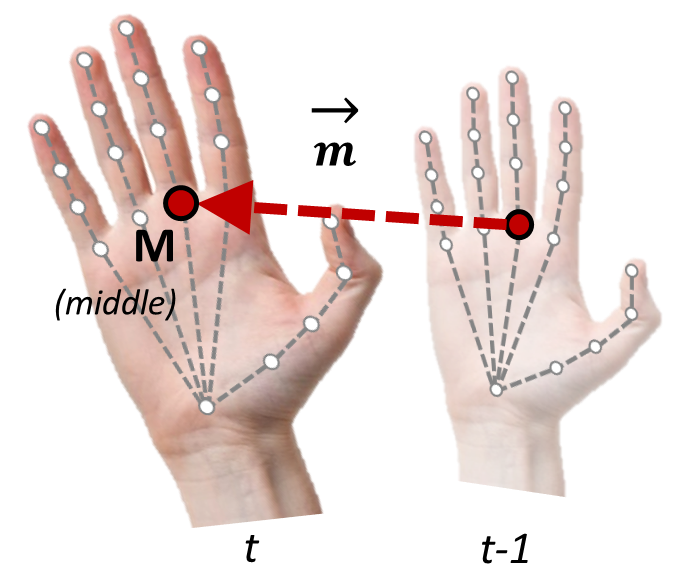
\includegraphics[height=4cm]{imagens/metodologia/datasets/hand_movement}
        }%
        \hspace{1cm}
        \subcaptionbox{\label{subfig:hand-directions}}{
            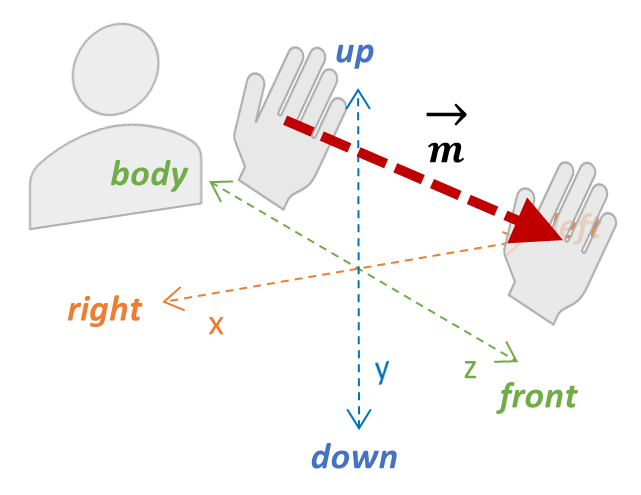
\includegraphics[height=4cm]{imagens/metodologia/datasets/hand_movement_2}
        }%
        \nomefonte{}
        \label{fig:hand-movement-directions}
    \end{figure}


    A partir do vetor \(\overrightarrow{m}\), aplicamos uma operação parecida com a que foi utilizada para a orientação da mão, para definir o movimento da mão \(V_{hand}\) como a combinação de até três direções, cujas opções são: \textit{right} (direita), \textit{left} (esquerda), \textit{up} (para cima), \textit{down} (para baixo), \textit{body} (para o corpo) ou \textit{front} (para frente). Essa operação é detalhada na \autoref{eqn:hand-movement-directions} e a \autoref{subfig:hand-directions} ilustra ela segundo a perspectiva do sinalizador:

    % Directions
    \begin{equation}
    \label{eqn:hand-movement-directions}
        V_{hand} =
            \begin{cases}
                right & \text{if $\overrightarrow{m}_x < {-k}$ }\\
                left  & \text{if $\overrightarrow{m}_x > {k}$ }\\
                up    & \text{if $\overrightarrow{m}_y < {-k}$ }\\
                down  & \text{if $\overrightarrow{m}_y > {k}$ }\\
                body  & \text{if $\overrightarrow{m}_z < {-k}$ }\\
                front & \text{if $\overrightarrow{m}_z > {k}$ }\\
            \end{cases}    
    \end{equation}

    Aqui o limiar \(k\) também foi definido como 0,30 para remover movimentos pouco significantes.


    % -----
    \item \textbf{Expressão não-manual - abertura da boca}:
    
    Para o atributo abertura da boca, consideramos a pesquisa desenvolvida por \cite{ferrario-2000-study-lips}, que analisa e estabelece alguns parâmetros de referência para os lábios humanos.

    % A partir desses parâmetros, selecionamos o \textit{largura altura-boca do vermelhão} porque ele pode medir os lábios em termos de uma única relação (entre a altura do vermelhão e a largura da boca, como em \autoref{fig:abertura da boca }). Assim, a altura do vermelhão é a distância \(d\) entre o labiale superius \(LS\) e o labiale inferius \(LI\), que são os pontos-chave mais externos dos lábios superior e inferior. A largura da boca, por sua vez, é a distância \(d\) entre o cheilion direito \(CH_r\) e o cheilion esquerdo \(CH_l\), que são os pontos-chave do lado direito e esquerdo da boca~\cite{ ferrario2000normal}.

    \figura
        {fig:mouth-openness} % Label
        {imagens/metodologia/datasets/mouth_openness} % Path
        {height=4cm} % Size
        {A abertura da boca foi calculada com base no parâmetro \textit{largura altura-boca do vermelhão} apresentado por \cite{ferrario-2000-study-lips}, que é obtido a partir das coordenadas \(LS\), \(LI\), \(CH_r\) e \(CH_l\).} % Caption
        {ferrario-2000-study-lips} % Citation

    Este cálculo acima foi adotado para determinar a abertura de boca \(P_{mouth}\), da seguinte forma:

    % Abertura da boca:
    \begin{equation}
        \label{eqn:mouth-openness}
        P_{mouth} = \frac{d(LS, LI)}{d(CH_r, CH_l)}
    \end{equation}

\end{enumerate}